\chapter{DAH Quiz}
\label{sec:quiz}

Solve the following questions about data acquisition and handling material on your own time,
i.e. you should not use the laboratory hours to solve the quiz questions. 
In total, 20 marks can be obtained.
The quiz will count for 10\% of the total course mark, see also the course booklet. 

Please hand in your solutions to the questions to the Teaching Office.

{\bf Deadline:} 12 noon, Tuesday, 5$^{th}$ November 2019.

\begin{enumerate}

\item  In a particle physics experiment at the Large Hadron Collider at CERN, photons  are recorded in an electromagnetic crystal calorimeter. Each crystal is read out with a photodetector and the signals
are  digitised with an Analog-to-Digital Converter (ADC).
%
\begin{itemize}
%\item With the aid of a diagram, explain briefly how an ADC works.
\item In order to measure photon  energies  in  the dynamic range of 40 MeV to  2.0 TeV,
how many bits are required for the ADC? 
%\item In practise, the energy deposited in a crystal is measured with multiple 12-bit ADC channels %which cover low and high energy ranges separately by using  a multi gain preamplifer, see figure.
%Show that the gain factors 1, 6 and 12 are sufficient to cover the full dynamic range.
\end{itemize}
[ Hint: 1 TeV = $10^{12}\; \rm eV$, 1 GeV = $10^9\; \rm eV$ and 1 MeV = $10^6\; \rm eV\; .$ ]
%
\hfill {\bf [2 marks]}\\

%\begin{comment}
\item In DAH checkpoint (4) a PCF8574AN expander I/O chip was used to control a LED light pattern.  You were instructed to connect all address lines (A0, A1, A2) to ground which corresponds to the slave address {\tt 0x38}. What would the slave address be  if all address lines were connected to 3.3V?
Explain hexadecimal numbers. 

The I2C bus allows to connect multiple slave devices. How many PCF8574AN chips can be controlled in total from one Raspberry-Pi?

[ Hint: You need to consult the PCF8574AN data sheet. 
Note that the prefix {\tt 0x} is used for representing numbers in hexadecimal notation.  ] 
%
\hfill {\bf [2 marks]}\\
%\end{comment}

\item Charged particles traversing a drift chamber, ionise the gas and the electrons drift toward anode wires where these are multiplied in a high electric field. Thus a fast charge signal is produced which can be converted into a voltage pulse by means of a pre-amplifier. 
The drift time is a measure of the distance from where the the drift electrons were created to the anode wire.

In a particle physics experiment, a drift chamber with 384~anode wires is used to measure trajectories of charged particles. 
The drift velocity is $1\; {\rm cm/\mu s}$, the maximum drift time is $6.5 \; \mu$s
and  a spatial resolution of  better than $200\; \mu$m is needed.
What electronics equipment is required to read out the signal pulses of the drift chamber? State its main specifications.
\hfill {\bf [5 marks]}\\

\item The $^{22}$Na nuclei decays with a half-life of 2.6 years by positron emission. The positron annihilates with an electron giving rise to a pair of $\gamma$-rays with energies of 0.51 MeV. 
Coincidence measurements can be used to demonstrate that two 0.51 MeV $\gamma$-rays are produced  with the two photons travelling in opposite directions. A schematic  of the apparatus you might use to record the pairs of photons is shown below:
%
\begin{center}
 {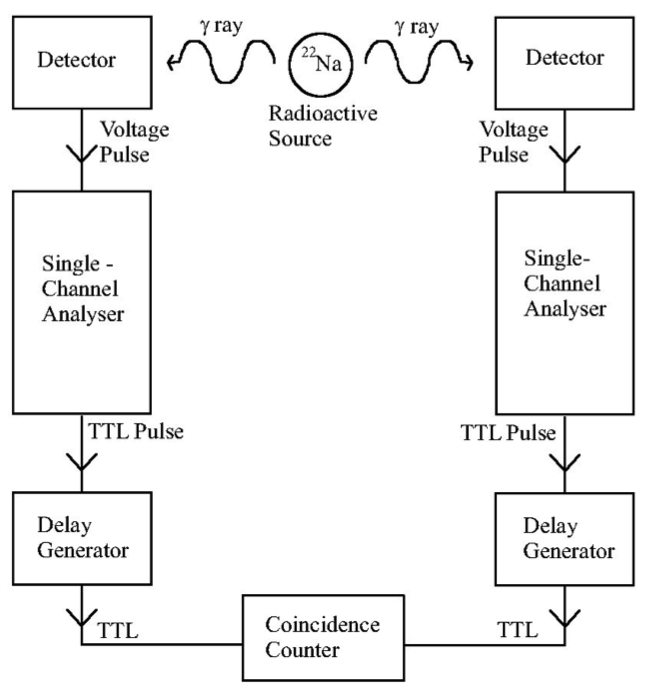
\includegraphics[width=0.35\textwidth]{figs/positron-annihilation}}
 \end{center}
%
The pulses from the detector have a peak voltage that is proportional to the energy of the $\gamma$-rays. By means of  a  single-channel analyser  a TTL pulse is  produced whenever the amplitude of the input pulse lies within a specified voltage range.
\begin{itemize}
\item With the aid of a diagram show the sequence of pulses from the detector to the coincidence unit, illustrating how a single-channel analyser works.  What does TTL stand for?
What does this imply about the output pulses of the single-channel analyser?
\item Delay generators can be used to delay the time at which one of the pulses reaches the coincidence counter.
Explain why this might be necessary. % to delay one of the pulses.
%
%\item 
%To determine whether two pulses are coincident, what logic operation is required?
\hfill {\bf [4 marks]}
%
\end{itemize}



\item A peak  in a data distribution, which is clearly visible (by eye) can usually be assigned to a signal (e.g. a particle mass, an atomic transition wavelength, ...). 

Explain what  the  resolution ($\sigma$) and the Full Width Half Maximum (FWHM)  of a signal peak in a distribution are. 
Derive the relation, FWHM$  = 2 \sqrt{2 \log 2}\; \sigma$, for the resolution $\sigma$ of a Gaussian distribution.  
\hfill {\bf [3 marks]}\\

Write a python script which uses random numbers to generate a Gaussian distribution with a mean $\mu$ and a resolution $\sigma$.
Plot a histogram of  this distribution.
Calculate the mean and variance  of the generated distribution and show 
that the results agree with your input values.
You need to submit a printout of your code and its outputs.

%[ Hint: For random numbers, use the python notes, available on Learn. ]
\hfill {\bf [4 marks]}



\begin{comment}
\item Write a short python script which generates a flat distribution and plots a histogram of  
the distribution.
Calculate the mean and variance  of the generated distribution and show that for a flat distribution between $a$ and $b$, the relation
 $\sigma = \frac{b-a}{\sqrt{12}}$  for the resolution $\sigma$ 
is satisfied. You need to submit a printout of your code.

Derive the  relation $\sigma = \frac{b-a}{\sqrt{12}}$ for the resolution $\sigma$ of a flat distribution between $a$ and $b$.  

\hfill {\bf [6 marks]}
\end{comment}

\end{enumerate}